\documentclass[12pt]{article}
\usepackage[utf8]{inputenc}
\usepackage{float}
\usepackage{amsmath}
\usepackage{graphicx}
\usepackage{enumitem}

\usepackage[hmargin=3cm,vmargin=6.0cm]{geometry}
\topmargin=-2cm
\addtolength{\textheight}{6.5cm}
\addtolength{\textwidth}{2.0cm}
\setlength{\oddsidemargin}{0.0cm}
\setlength{\evensidemargin}{0.0cm}
\usepackage{indentfirst}
\usepackage{amsfonts}

\begin{document}

\section*{Student Information}

Name : Emre Geçit

ID : 2521581

\section*{Question 1}
Design a Turing machine which recognizes the language $L = \{0^N1^N | N \geq 1\}$.

$\Sigma = \{0, 1, \sqcup\}$, means that you cannot write any other symbol than these symbols.
\subsection*{States:}
\begin{itemize}
    \item State 0 (Initial state): If the tape head is on a 0, changes it with a blank space, moves the tape head to right, and passes to the state 1. If it is on a blank space, passes to the acceptance state.
    \item State 1: This state's task is finding the right end of the string. After finding the rightmost symbol in the string, the machine passes to state 2.
    \item State 2: If the tape head is on a 1, changes it with a blank space, moves the tape head to left, and passes to the state 3. If it is on a blank space, passes to the acceptance state.
    \item State 3: This state's task is finding the left end of the string. After finding the leftmost symbol in the string, the machine passes to state 0.
\end{itemize}
Note that in these descriptions, undefined transititons leads to rejection of the string.
\begin{figure}[H]
    \caption{Turing machine which recognizes the language $L = \{0^N1^N | N \geq 1\}$}
    \centering
    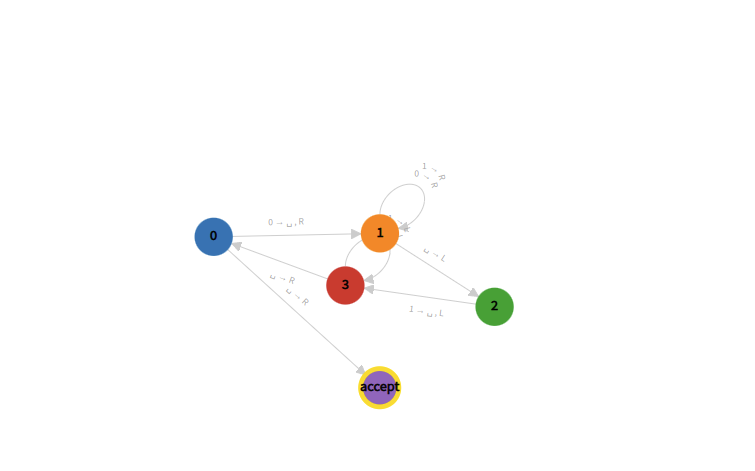
\includegraphics[width=12cm]{Q1/turingmachine.io_.png}    
\end{figure}
\newpage
\subsection*{Sample inputs:}
\begin{figure}[H]
    \caption{Input = 000111}
    \centering
    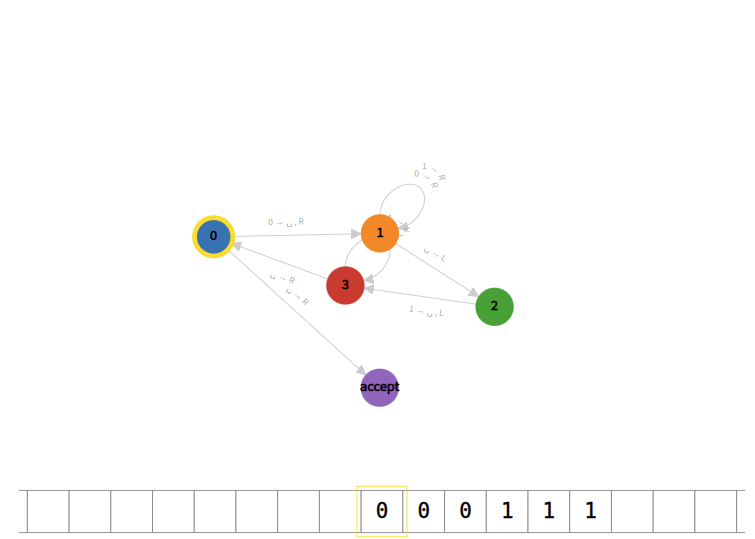
\includegraphics[width=12cm]{Q1/000111.png}    
\end{figure}
\begin{figure}[H]
    \caption{000111 accepted}
    \centering
    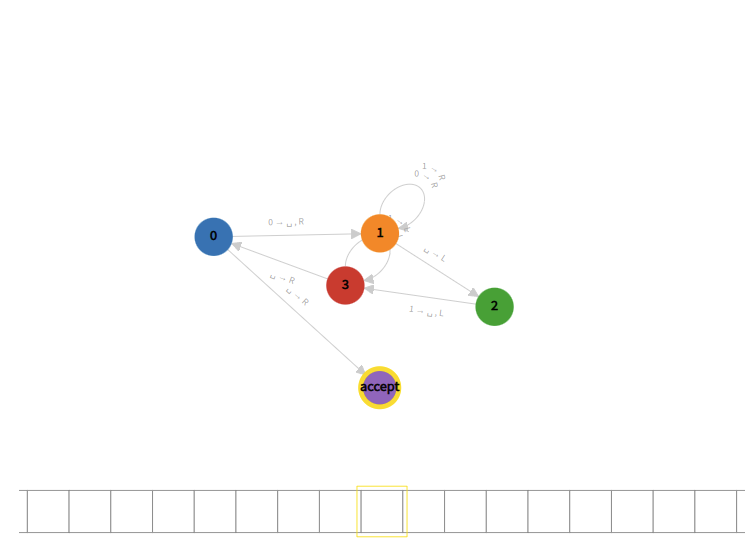
\includegraphics[width=12cm]{Q1/000111o.png}    
\end{figure}
\begin{figure}[H]
    \caption{Input = 0000111}
    \centering
    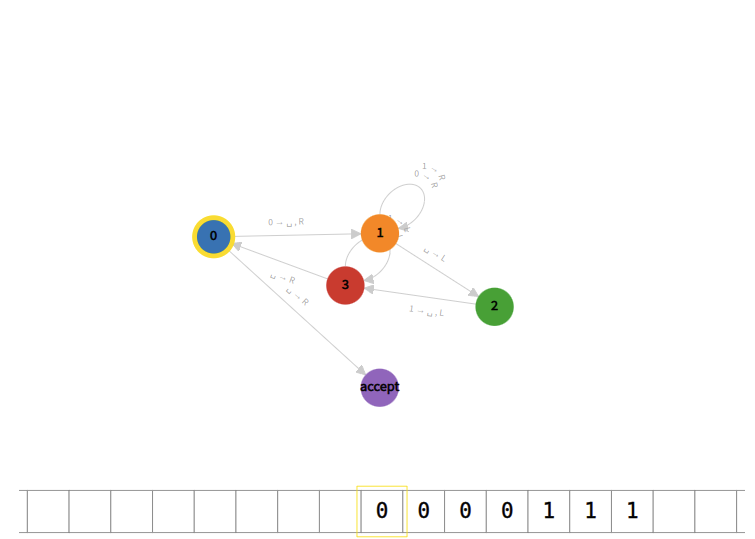
\includegraphics[width=12cm]{Q1/0000111.png}    
\end{figure}
\begin{figure}[H]
    \caption{0000111 rejected}
    \centering
    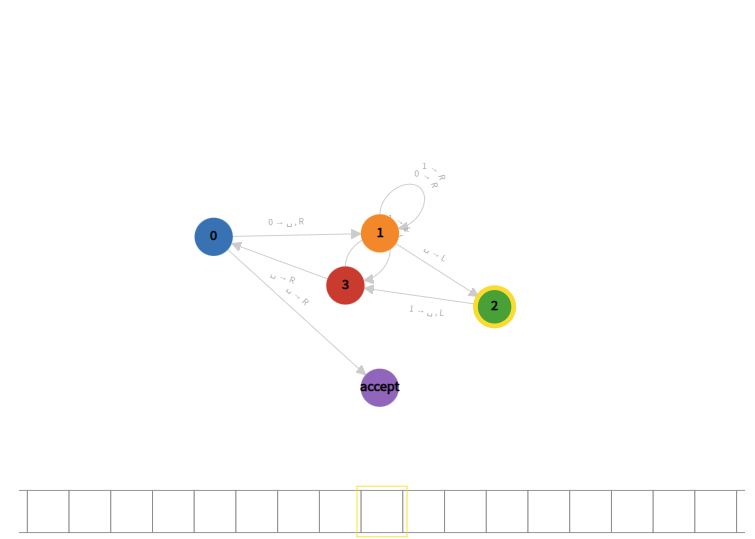
\includegraphics[width=12cm]{Q1/0000111o.png}    
\end{figure}
\begin{figure}[H]
    \caption{Input = 000011111}
    \centering
    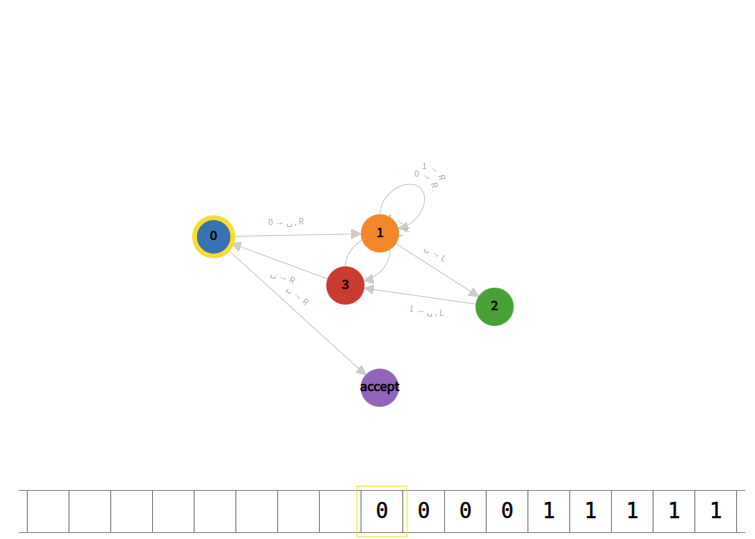
\includegraphics[width=12cm]{Q1/000011111.png}  
\end{figure}
\begin{figure}[H]
    \caption{000011111 rejected}
    \centering
    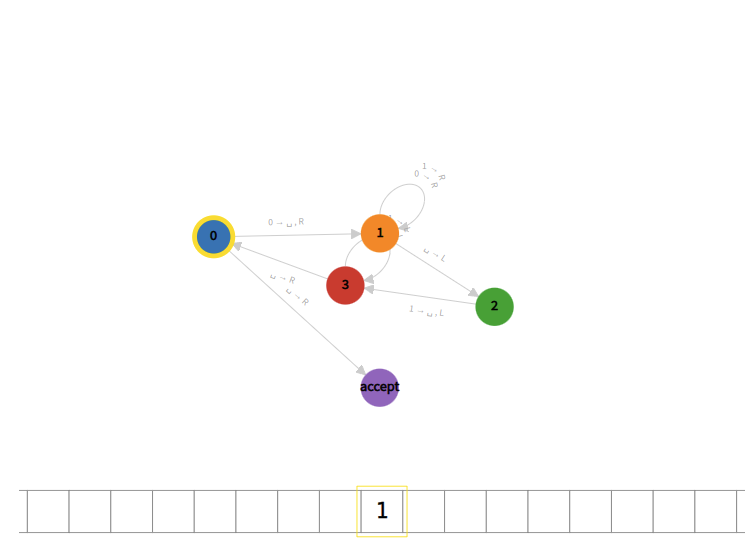
\includegraphics[width=12cm]{Q1/000011111o.png}  
\end{figure}
\begin{figure}[H]
    \caption{Input = 0001110}
    \centering
    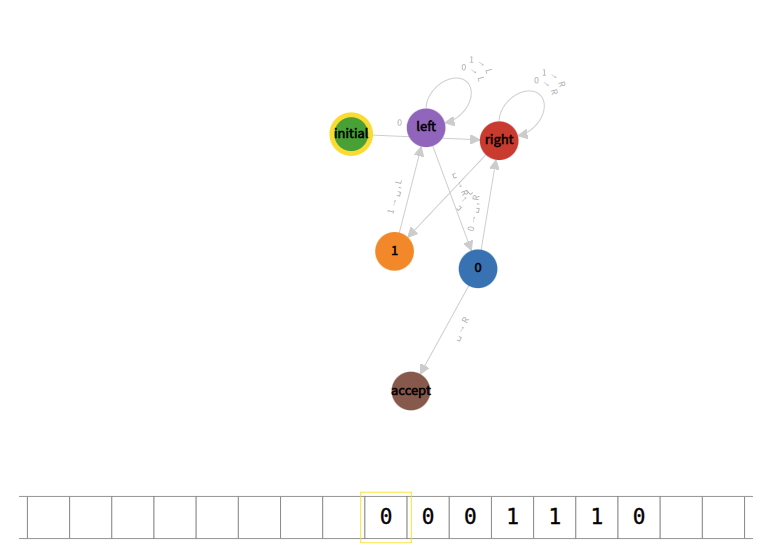
\includegraphics[width=12cm]{Q1/0001110.png}  
\end{figure}
\begin{figure}[H]
    \caption{0001110 rejected}
    \centering
    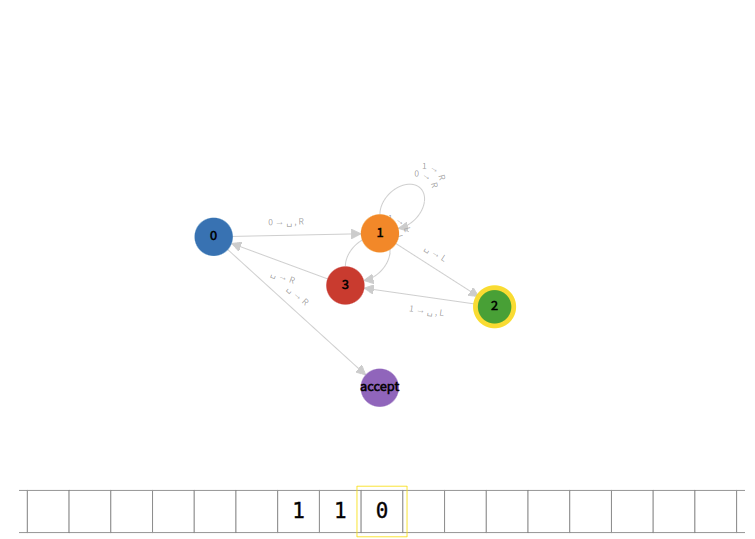
\includegraphics[width=12cm]{Q1/001101o.png}  
\end{figure}
\begin{figure}[H]
    \caption{Input = 100011}
    \centering
    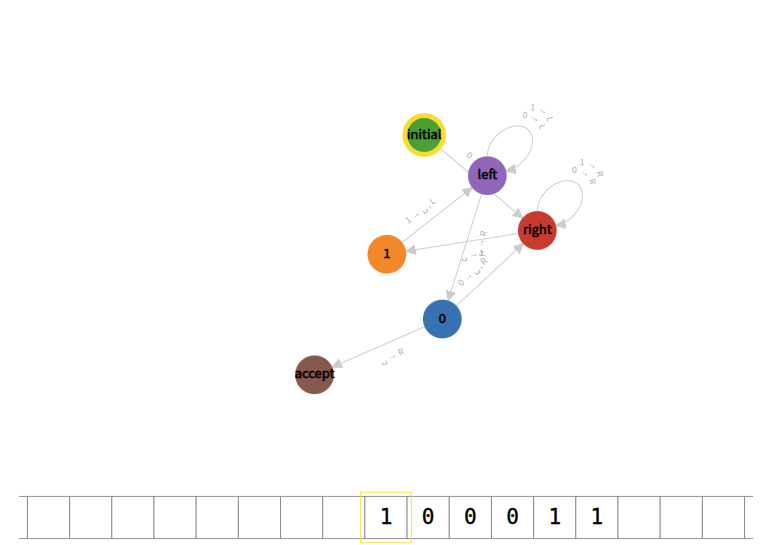
\includegraphics[width=12cm]{Q1/100011.png}
\end{figure}
\begin{figure}[H]
    \caption{100011 rejected}
    \centering
    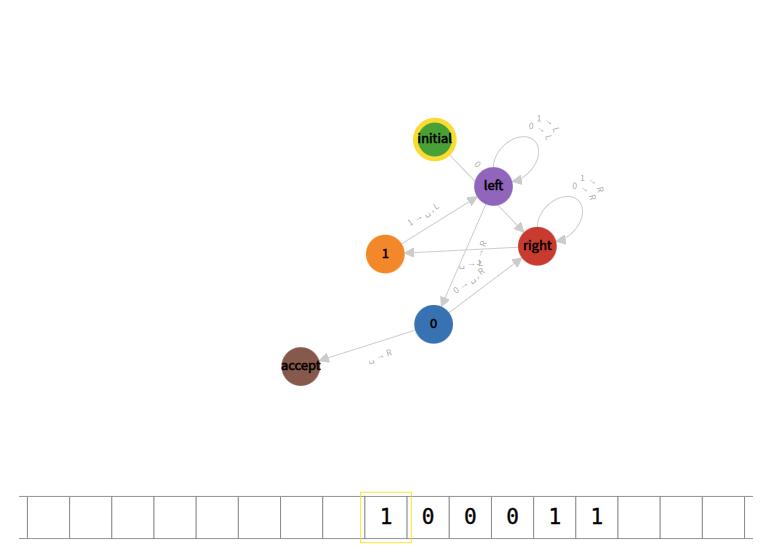
\includegraphics[width=12cm]{Q1/100011o.png}
\end{figure}
\newpage
\section*{Question 2}
Design a Turing machine that computes the function $f(w) = ww^R$, $\Sigma(w) = \{0, 1\}$.
\subsection*{States:}
\begin{itemize}
    \item convert{\_}symbols (Initial state): This states changes all zeros with x's, and all ones with y's. Then, it moves the tape head to the right.
    \item find{\_}last{\_}character: This state finds the last symbol that has not been copied and passes to copy{\_}y if the tape head is on a y, or to copy{\_}x if the tape head is on a x.
    \item copy{\_}y: This state goes to the end of the tape, and writes a 1.
    \item copy{\_}x: This state goes to the end of the tape, and writes a 0.
\end{itemize}
\begin{figure}[H]
    \caption{Turing machine which computes the function $f(w) = ww^R$}
    \centering
    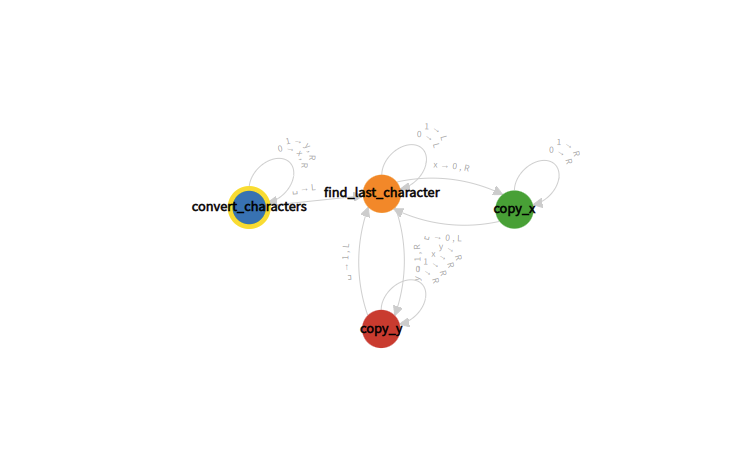
\includegraphics[width=17cm]{Q2/turingmachine.io_.png}
\end{figure}
\newpage
\subsection*{Sample inputs:}
\begin{figure}[H]
    \caption{Input = 1011}
    \centering
    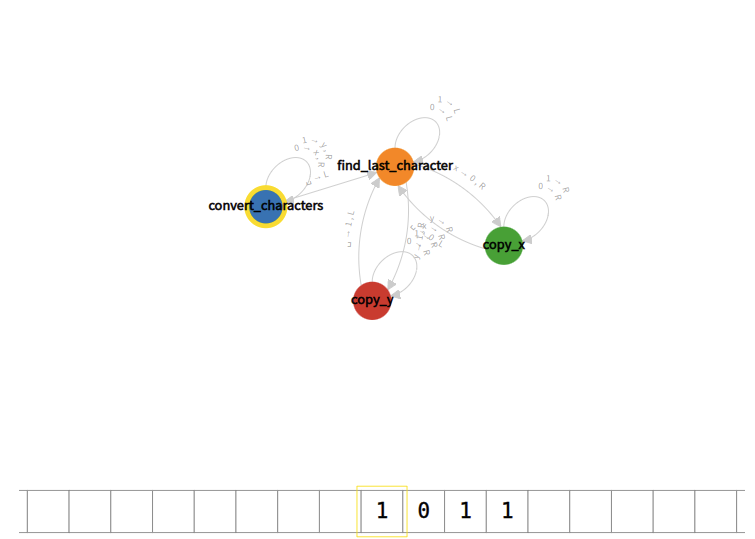
\includegraphics[width=12cm]{Q2/1011.png}
\end{figure}
\begin{figure}[H]
    \caption{Output = 10111101}
    \centering
    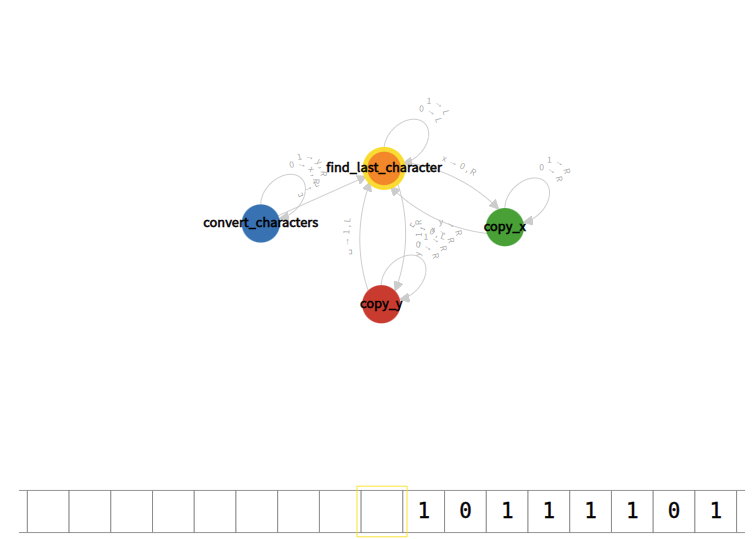
\includegraphics[width=12cm]{Q2/10111101.png}
\end{figure}
\begin{figure}[H]
    \caption{Input = 1110}
    \centering
    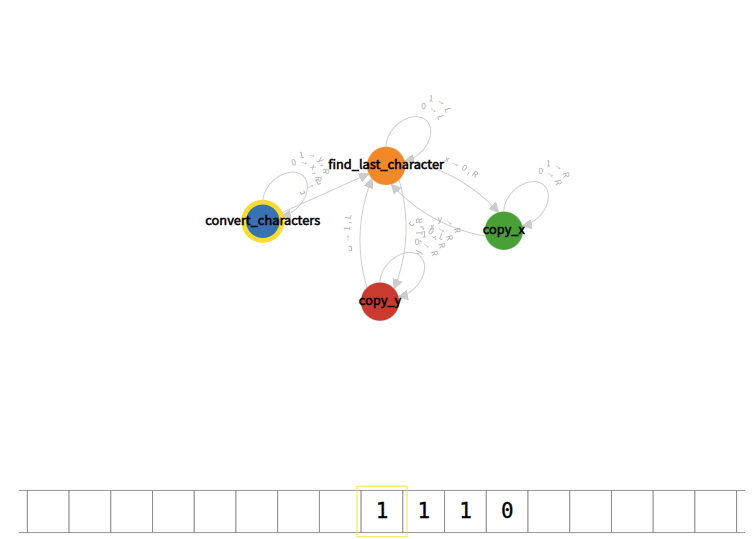
\includegraphics[width=12cm]{Q2/1110.png}
\end{figure}
\begin{figure}[H]
    \caption{Output = 11100111}
    \centering
    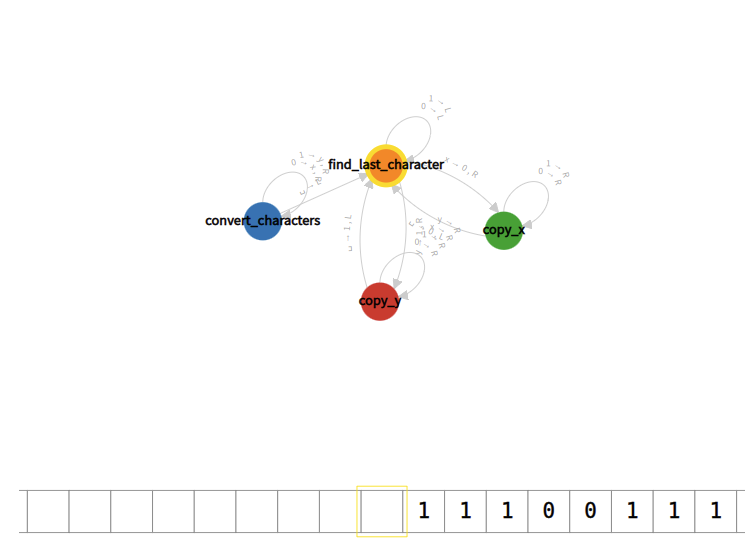
\includegraphics[width=12cm]{Q2/11100111.png}
\end{figure}
\begin{figure}[H]
    \caption{Input = 0101}
    \centering
    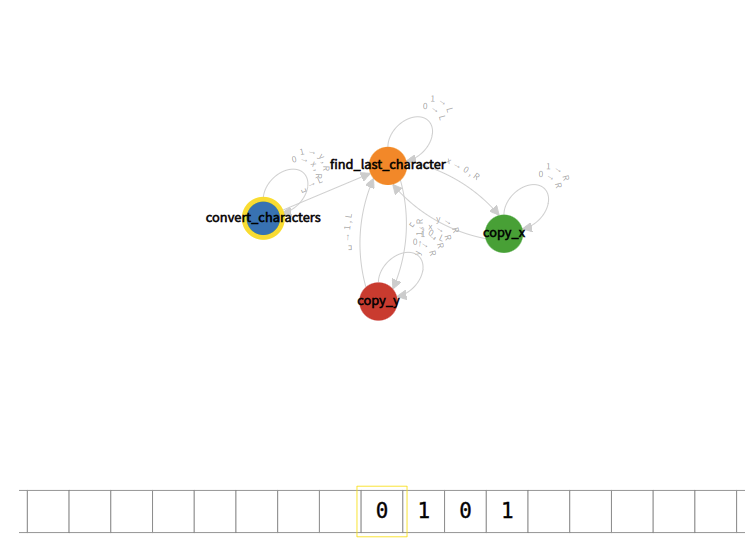
\includegraphics[width=12cm]{Q2/0101.png}
\end{figure}
\begin{figure}[H]
    \caption{Output = 01011010}
    \centering
    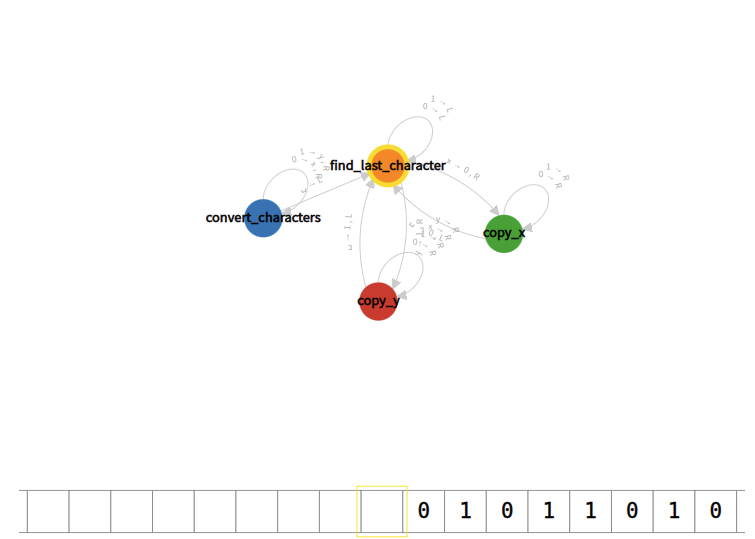
\includegraphics[width=12cm]{Q2/01011010.png}
\end{figure}
\begin{figure}[H]
    \caption{Input = 1010}
    \centering
    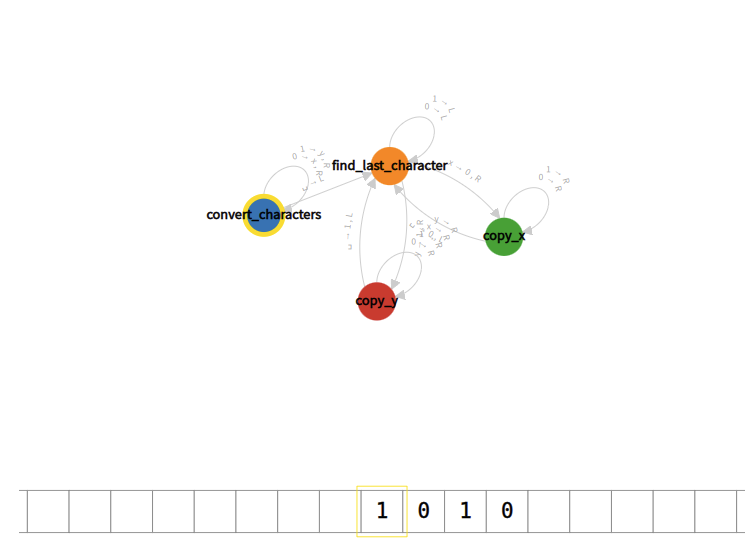
\includegraphics[width=12cm]{Q2/1010.png}
\end{figure}
\begin{figure}[H]
    \caption{Output = 10100101}
    \centering
    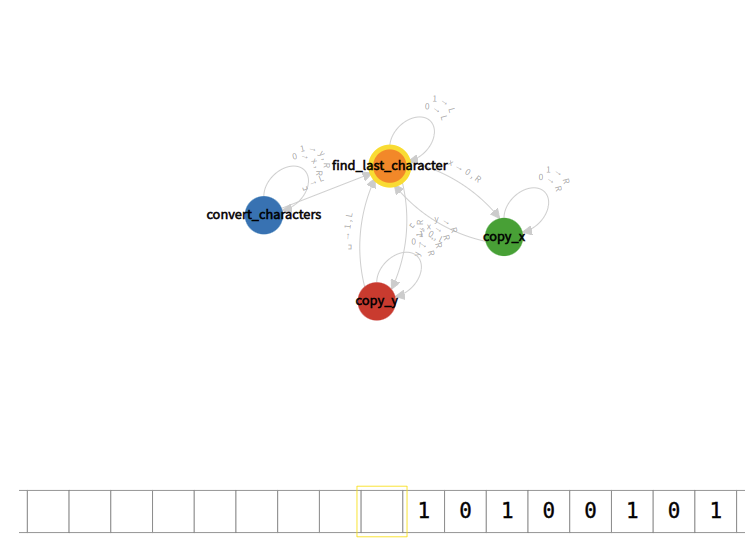
\includegraphics[width=12cm]{Q2/10100101.png}
\end{figure}
\begin{figure}[H]
    \caption{Input = 1010001}
    \centering
    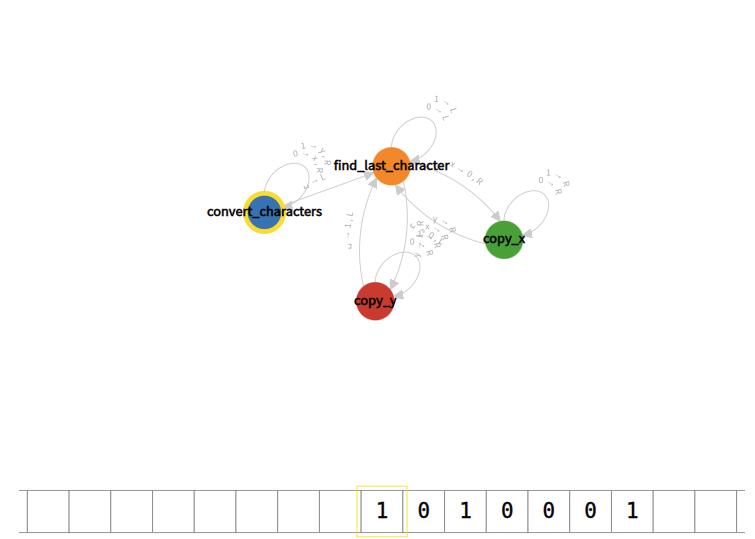
\includegraphics[width=12cm]{Q2/1010001.png}
\end{figure}
\begin{figure}[H]
    \caption{Output = 10100011000101}
    \centering
    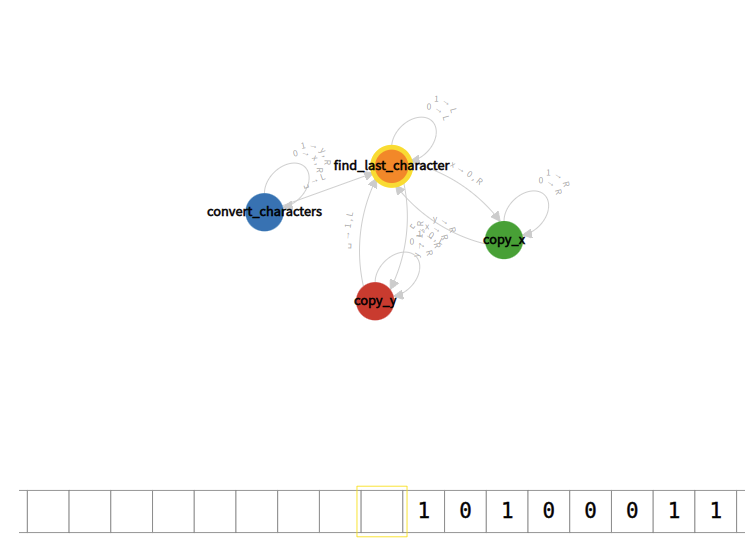
\includegraphics[width=12cm]{Q2/10100011000101.png}
\end{figure}
\begin{figure}
    \caption{Input = 00111}
    \centering
    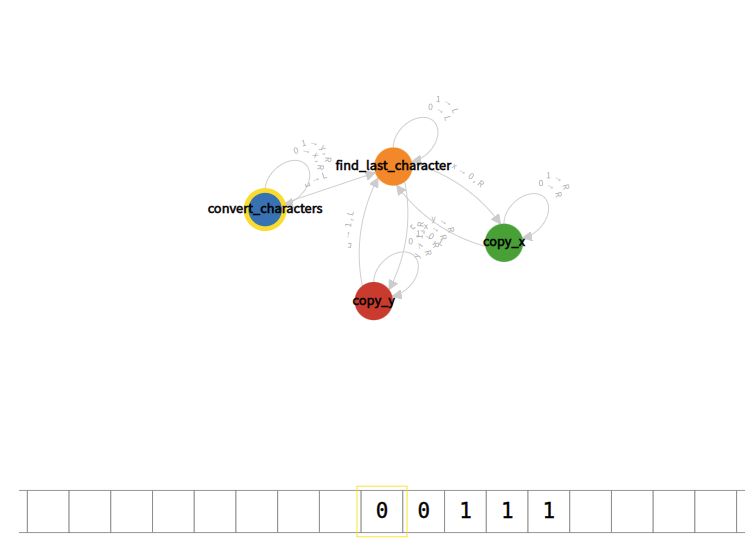
\includegraphics[width=12cm]{Q2/00111.png}
\end{figure}
\begin{figure}
    \caption{Output = 0011111100}
    \centering
    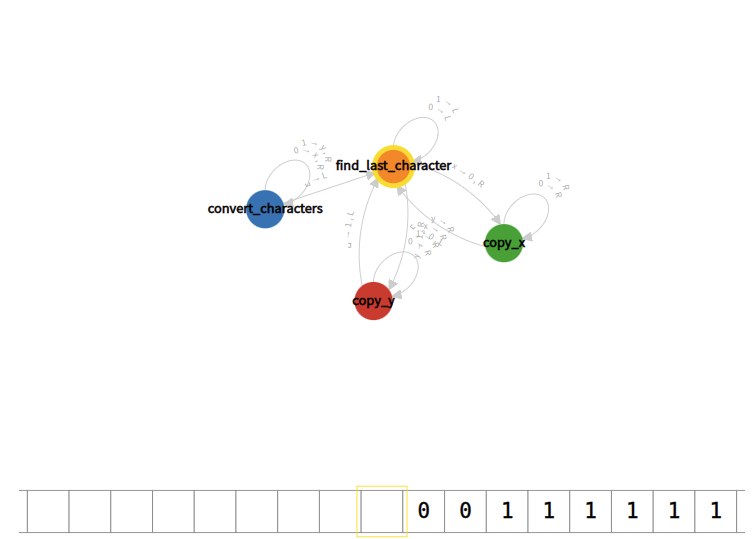
\includegraphics[width=12cm]{Q2/0011111100.png}
\end{figure}
\newpage
\section*{Question 3}
Formally define a Turing machine with a 2-dimensional tape, its configurations, and its computation.
Define what it means for such a machine to decide a language L. Show that t steps of this machine,
starting on an input of length n, can be simulated by a standard Turing machine in time that is
polynomial in t and n.
\subsection*{Solution:}
\paragraph{1)} A Turing machine with a 2-dimensional tape is a pentuple $(K, \Sigma, \delta, s, H)$, where

\begin{itemize}
    \item $K$ is a finite set of states;
    \item $\Sigma$ is a finite set of symbols containing the blank symbol $\sqcup$ but not containing $\uparrow$, $\rightarrow$, $\downarrow$ or $\leftarrow$;
    \item $s\in K$ is the initial state;
    \item $H \subseteq K$ is the set of halting states;
    \item $\delta$, the transititon function, $\delta: (K - H) \times  \Sigma \to (K - H) \times (\Sigma \cup \{\uparrow, \rightarrow, \downarrow, \leftarrow\})$ such that,
\end{itemize}
\begin{enumerate}[label=(\alph*)]
    \item for all $q \in K-H$, if $\delta(q, \vartriangleright) = (p, b)$, then $b = \rightarrow$
    \item for all $q \in K-H$, if $\delta(q, \bigtriangledown) = (p, b)$, then $b = \downarrow$
    \item for all $q \in K-H$ and $a \in \Sigma$, if $\delta(q, a) = (p, b)$, then $b \neq \vartriangleright$ and $b \neq \bigtriangledown$
\end{enumerate}

A configuration of a Turing machine with a 2-dimensional tape is
\begin{center}
    $K \times N \times N \times T$,
\end{center}
Where $T$ is the set of functions from $N \times N$ to $\Sigma$, that have $t(0, y) = \vartriangleright$ and $t(x, 0) = \bigtriangledown$ for all $x, y \in \mathbb{N}$ and have $t(x, y)$ = for all but a finite number of $(x, y)$ pairs. Thus, we represent a configuration by the current state, current head position, and a list of all non-blank squares on hte tape.

Given a string w, let $t_w\in T$ be the function that has $t(i+1, 1) = w(i)$ for $0 < i \leq |w|$, $t(0, y) = \vartriangleright$ for $y\in \mathbb{N} $, $t(x, 0) = \bigtriangledown$ for all $x > 0$ and $t(x, y) = \sqcup$ otherwise. Then if we have a two-dimensional tape Turing machine M with two distinguished halting states y and n such that for any string $w$ either $(s, 1, 1, t_w) \vdash^*_M (y, i, j, t')$ or $(s, 1, 1, t_w) \vdash^*_M (n, i, j, t')$ for some $i, j$ and $t'\in T$, we let the language decided by M be the set of strings for which M thus halts in the y state.

From the definition of $T$, any $t \in T$ can be encoded as a finite set of ordered triples $(x, y, \sigma)$. If we encode these values along a tape, we can use dovetailing to assign a unique square for each possible $x, y$ value. We then fill in the non-blank entries of $t$ in this tabular format, so that $t(x, y)$ is stored in the $\dfrac{(i+j)^2+3i+j}{2}$th square. At any time during the computation, only finitely many squares of this encoding tape will be non-blank.

Therefore, we simulate $M$ with a three-tape Turing machine $M'$. $M'$ uses one tape for calculation, one to hold the encoding of the tape of $M$ as described above, and takes its input on the third. The calculations $M$ needs to perform are as follows:
\begin{enumerate}
    \item increment and decrement two registers, $i$ and $j$
    \item simple multiplications and additions
\end{enumerate}

In each step of the computation, $M'$ looks at the current symbol on the encoding tape and at the current state of $M$. If the instrucions are to write a symbol, $M'$ writes that symbol and proceeds. If the instrucions are to move, $M'$ increments or decrements $i$ or $j$ as appropriate, then calculates the value of the dovetail function. $M'$ then moves the encoding-tape head all the way to the left, then out to the appropriate square.

At any time, if $i$ and $j$ represents the largest $x$ and $y$ coordinates that $M$ has been in, then neither $i$ or $j$ is larger than $t$. Thus the process of simulating one move takes the time required to increment or decrement a binary register, compute some binary sums and products, and move one head by a number of spaces that is a quadratic polynomial in $i$ and $j$, and thus is bounded by a quadratic polynomial in $t$. The increments and arithmetic are fast, and can be done in polynomial time in $t$. Thus the time to carry out $t$ steps, once we have finished the initial setup, is $\mathcal{O}(t^3)$. The initial setup consists copying out the tape of $M$ into its $M'$ and takes 2n-step computation of alternating writes and moves, so that it can be carried out in time $\mathcal{O}(n^3)$ by the same reasoning. Thus the overall simulation proceeds in time polynomial in $t$ and $n$.

Up to here, we assumed that there will be a finite number of non-blank squares. But theoretically, the tile of the 2d-tape can be filled infinitely, and there can be an infinite number of non-blank squares. In that case, the Turing machine will fail halting, and can never be simulated. Considering this possibility, I offer a continuing the copying process, as the computation proceeds, instead of first copying the tape, and than doing the simulation. That is, in each state, if the read square on the encoding tape, if the read square is blank, enter another state, copy the corresponding symbol, and continue the computation. With this process, we need to be careful when copying a blank symbol from the 2d-tape, to the encoding tape. In order not to enter in an infinite loop, when copying a blank symbol, we need to write a special symbol to the encoding tape. This new algorithm runs in a similar time as the original algorithm, but it works with tapes that have infinitely many non-blank squares.
\end{document}